\documentclass[12pt,a4paper]{article}

\usepackage[utf8]{inputenc}
\usepackage[english]{babel}
\usepackage{amsmath}
\usepackage{amsfonts}
\usepackage{amssymb}
\usepackage{graphicx}
\usepackage{lmodern}
\usepackage[left=2cm,right=2cm,top=2cm,bottom=2cm]{geometry}

\usepackage{siunitx}
\usepackage{enumitem}
\usepackage[skip=.38\baselineskip]{parskip}
\usepackage{xcolor}   % for \textcolor
\usepackage{listings}
\definecolor{mGreen}{rgb}{0,0.4,0.1}
\definecolor{mGray}{rgb}{0.5,0.5,0.5}
\definecolor{mPurple}{rgb}{0.58,0,0.82}
\definecolor{backgroundColour}{rgb}{0.95,0.95,0.92}
\lstset{
	%backgroundcolor=\color{backgroundColour},   
    commentstyle=\color{mGreen},
    keywordstyle=\color{magenta},
    numberstyle=\tiny\color{mGray},
    stringstyle=\color{mPurple},
    %breakatwhitespace=false,                        
    %captionpos=b,
    %keepspaces=true,                 
    numbers=left,                    
    numbersep=5pt,                  
    showspaces=false,                
    showstringspaces=false,
    showtabs=false,                  
    %tabsize=8,	
    language=C,    
  	basicstyle=\small\ttfamily,
  	columns=fullflexible,
  	frame=single,
  	breaklines=true,
  	postbreak=\mbox{\textcolor{red}{$\hookrightarrow$}\space},
}

% for multi-figures
\usepackage{subcaption}

\usepackage{tabularx}
\usepackage{multirow}

% for graphs
%\usepackage{tikz}
%\usepackage{tkz-graph}
%\input{tkz-graph-patch}
%\usepackage{tikz-qtree}
%\usetikzlibrary{calc, arrows, positioning}

% custom commands
\newcommand{\multilinecell}[1]{\begin{tabular}{@{}c@{}}#1\end{tabular}}

\author{Olivér Facklam}
\title{CS473: Avalon slave laboratory\\Calculator through custom UART controller}

\newcommand{\nil}{\textit{nil}}

\begin{document}
\maketitle
\tableofcontents

\section{Problem statement}

The goal of this project is to create a simple text-based calculator supporting additions, using a custom UART controller as input/output mechanism.

The UART controller must be designed as an Avalon slave peripheral, allowing to integrate it onto the FPGA. It must be able to communicate with an external device through the UART protocol on a pair of TX/RX pins. The controller should also support configurable baud rate and parity settings.

The ``calculator'' application must receive an arithmetic expression (consisting of a single addition), parse it, and send the result back to the external device's terminal for display. All this communication must happen through the custom UART controller.


\section{System overview}

The overall system consists of 3 components: the NIOS-II processor, an on-chip memory, and our custom UART controller. The latter is connected to the host computer through a pair of TX/RX pins and a UART-to-USB converter. The overview of the system is shown in figure \ref{fig:system}.

\begin{figure}[h]
	\centering
	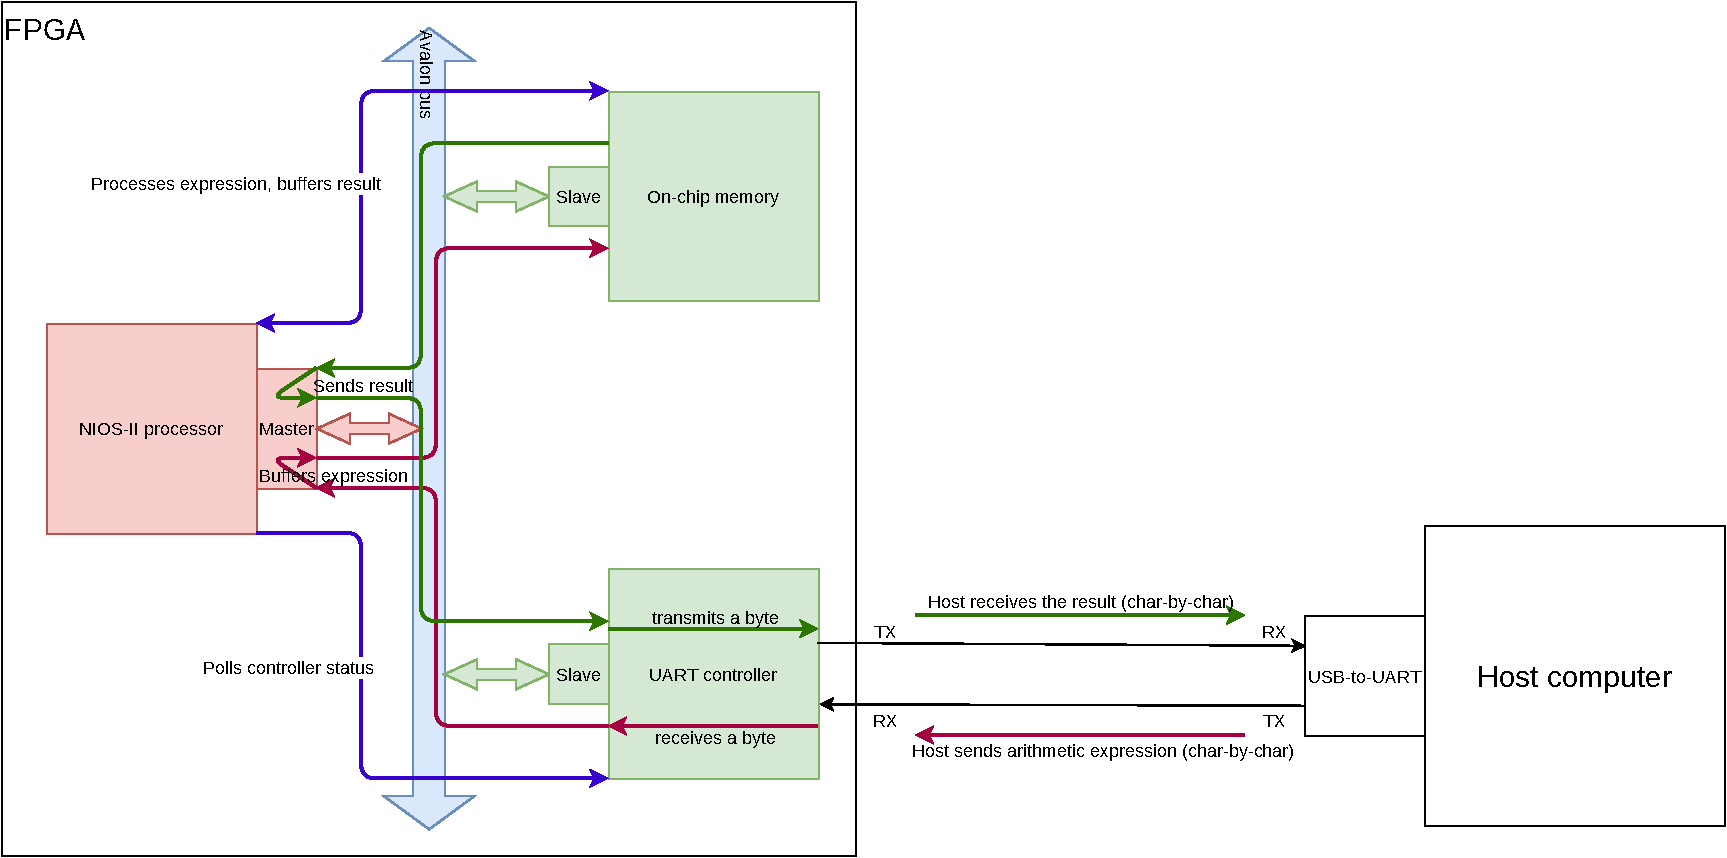
\includegraphics[width=\textwidth]{system}
	\caption{Overview of system architecture and operation}
	\label{fig:system}
\end{figure}

The standard operation of the application is the following:
\begin{enumerate}[nosep]
	\item The user types an arithmetic expression on the host terminal (used as an input device to the calculator).
	\item The host computer sends the sequence of bytes through the UART protocol to the controller on the FPGA.
	\item The UART controller receives these characters one-by-one, updating its status registers accordingly.
	\item The NIOS-II processor polls the controller to determine when new data has arrived, and buffers the received expression into memory.
	\item The processor parses the expression and prepares the response string, which is buffered into memory waiting for transmission.
	\item The processor polls the controller to determine when it is ready to transmit the next character, and sends the bytes one-by-one.
	\item The controller transmits each byte through the UART protocol to the host computer.
	\item The response is received by the host and displayed on the terminal (the output device of the calculator).
\end{enumerate}


\section{UART controller design}

In this section, we will describe the design and implementation of our custom UART controller. The goal is to create an Avalon memory-mapped slave peripheral, supporting configurable baud rate and parity, pollable status signals, and separate TX and RX buffers. The controller will then communicate using the UART protocol through a conduit consisting of a pair of TX/RX pins.

Some additional high-level design choices were made. The only supported data modes are:
\begin{itemize}[nosep]
	\item 8-bit data without parity and 1 stop bit (8N1 in minicom)
	\item 7-bit data with even parity and 1 stop bit (7E1)
	\item 7-bit data with odd parity and 1 stop bit (7O1).
\end{itemize}

In addition, a double-buffering system was chosen. This means that the controller doesn't have an internal FIFO; however it can store the next byte to transmit and the last byte received, while an active transmission and reception are going on.

\subsection{Programmable interface}

The physical interface of the peripheral is shown in figure \ref{fig:interface}. The controller has a clock and reset input, a memory-mapped slave interface, and a conduit for TX/RX.

\begin{figure}[h]
	\centering
	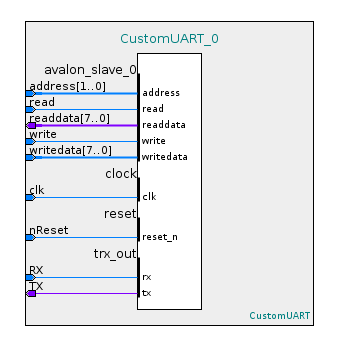
\includegraphics[width=.5\textwidth]{interface}
	\caption{Interface of the UART controller}
	\label{fig:interface}
\end{figure}

In table \ref{tab:map}, you can find the controller's register map.
We can see that the combined settings of clock divider (ranging from 1 to 128) and baud interval (ranging from 4 to 254 ticks/bit) allow -- assuming a \SI{50}{\mega\hertz} primary clock -- baud rates between 1.54 kBaud and 12.5 MBaud.

\begin{table}[ht]
	\centering
	\begin{tabularx}{\linewidth}{|c|c|c|X|}
		\hline
		Address & Register & Bits & Description \\
		\hline
		\hline
		\multirow{6}{*}{0x00} & \multirow{6}{*}{CTRL A} & 0 & \textbf{RX available} (read-only): set when a new received byte is available. \\
		 & & 1 & \textbf{TX ready} (read-only): set when the controller is ready to accept the next byte for transmission. \\
		 & & 2 & \textbf{parity enable}: 1 to enable the parity bit (7-bit data + 1 parity bit), 0 to disable (8-bit data). \\
		 & & 3 & \textbf{parity odd}: 1 to use odd parity, 0 to use even parity (ignored if parity is disabled). \\
		 & & 4 - 6 & \textbf{clock divider}: $\log_2$ of the clock divider value, i.e. values between 0-7 are mapped to dividers 1-128. Transmission and reception logic (including the baud rate setting) are with respect to the slow clock. \\
		 & & 7 & unused, always returns 0. \\
		 \hline
		 0x01 & CTRL B & 0-7 & \textbf{baud rate}: represents the baud interval in terms of slow clock ticks per bit. Only values $\geq$ 4 are accepted. Since this setting must be even, the LSB is always 0. \\
		 \hline
		 0x02 & RX DATA & 0-7 & \textbf{RX data} (read-only): last correctly received byte. Reading from this register also clears the \textit{RXavailable} flag \\
		 \hline
		 0x03 & TX DATA & 0-7 & \textbf{TX data}: next byte to transmit. Writing to this register also clears the \textit{TXready} flag.\\
		 \hline
	\end{tabularx}
	\caption{Register map of the UART controller}
	\label{tab:map}
\end{table}

\subsection{Internal architecture}

The internal architecture of the controller is depicted in figure \ref{fig:architecture}.

The architecture is composed of 4 major building blocks:
\begin{itemize}[nosep]
	\item a TX block (described in the next subsection);
	\item an RX block (described in the following subsection);
	\item a clock divider block, which simply takes as input a fast clock and a clock divider setting, and outputs a ``clock enable'' signal;
	\item a central ``logic'' block, composed of registers and a state machine, and which acts as the glue between these different entities and the avalon interface.
\end{itemize}

Several signals (\texttt{clkdiv}, \texttt{parityenable} and \texttt{parityodd} from the CTRL A register, and \texttt{baudrate} from the CTRL B register) are purely settings signals, and are directly fed into the appriopriate sub-entities. These are represented in yellow on figure \ref{fig:architecture}.

The signals in green on the figure, i.e. \texttt{TXdata}, \texttt{start}, \texttt{ready} and \texttt{TX} are the signals related to the TX dataflow. The signals in red, i.e. \texttt{RX}, \texttt{outputdata}, \texttt{dataok} and \texttt{RXdata} are related to the RX dataflow of the system.

Finally, the signals \texttt{TXready}, \texttt{RXavailable} (from CTRL A) and \texttt{newdata} (internal register) describe the state of the state machine. These are in purple on the figure \ref{fig:architecture}. The state machine itself is represented in figure \ref{fig:smsys}.


\begin{figure}[p]
	\centering
	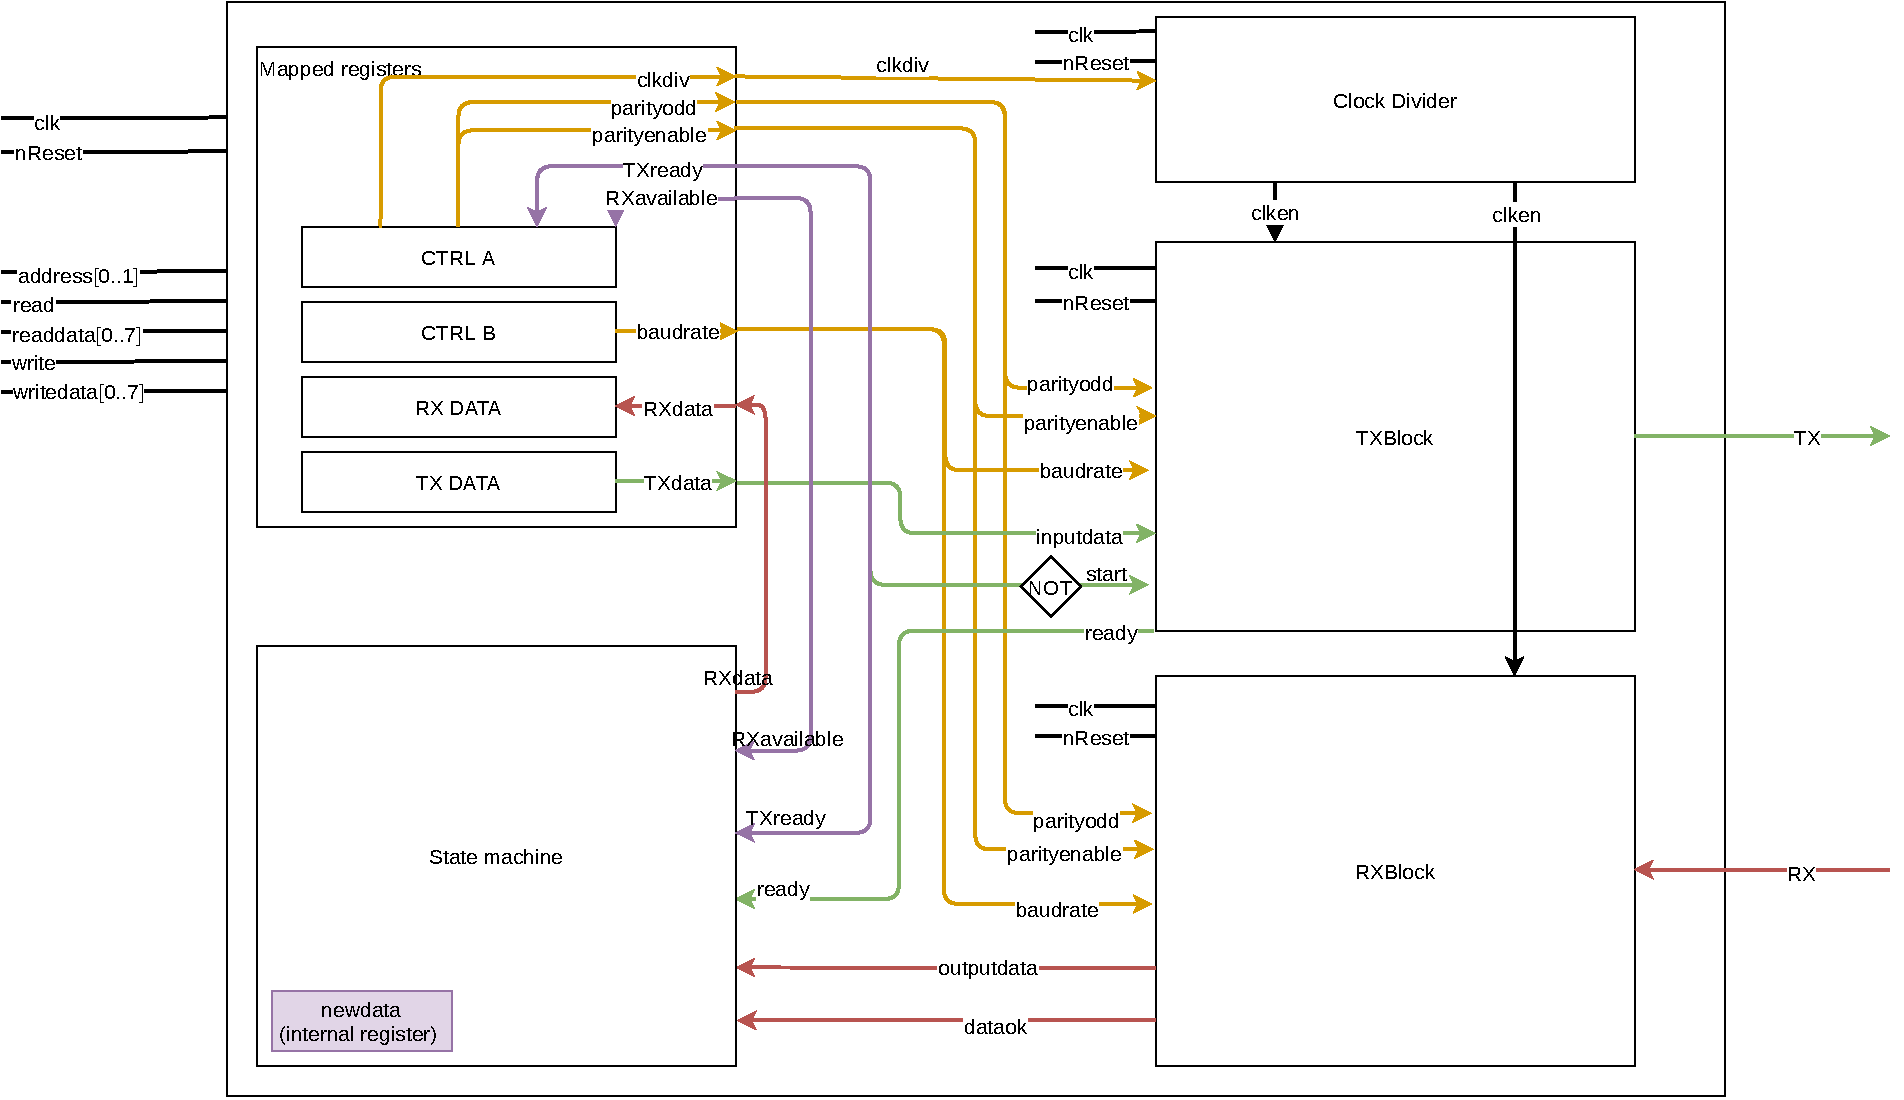
\includegraphics[width=\textwidth]{architecture}
	\caption{Architecture \& signals of the UART controller}
	\label{fig:architecture}
\end{figure}

\begin{figure}[p]
	\centering
	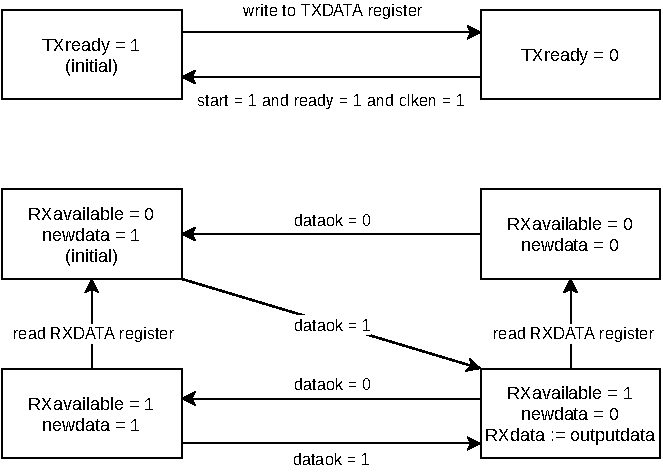
\includegraphics[width=.7\textwidth]{smsys}
	\caption{State machine of the UART controller logic}
	\label{fig:smsys}
\end{figure}

\subsection{TX design}

The job of the TX block is to transmit a single byte of data with the correct protocol and settings, over the TX line. Its interface and internal registers are summarized in figure \ref{fig:tx}.

The ready signal is used as an internal state, but is also exported for use in the controller logic. When a start signal is received in the idle state, the input data is copied into a local register, and the start bit is output on the TX pin. After this initial setup, each data bit is output at the configured baud interval. If necessary, the parity bit is also sent. Finally, a stop bit is output on the TX line for a whole baud interval before returning to the idle state. A summary of this state machine is shown in figure \ref{fig:smtx}. The whole TX logic is synchronous to the slow clock.

\begin{figure}[p]
	\centering
	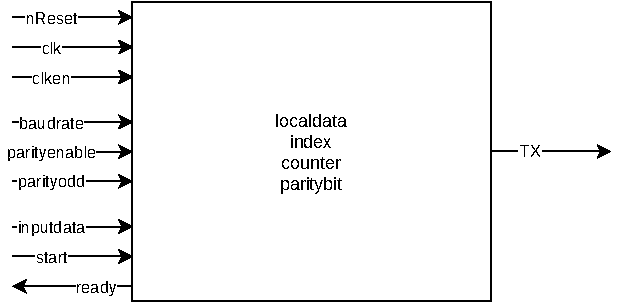
\includegraphics[width=.7\textwidth]{tx}
	\caption{Signals in the TX block}
	\label{fig:tx}
\end{figure}

\begin{figure}[p]
	\centering
	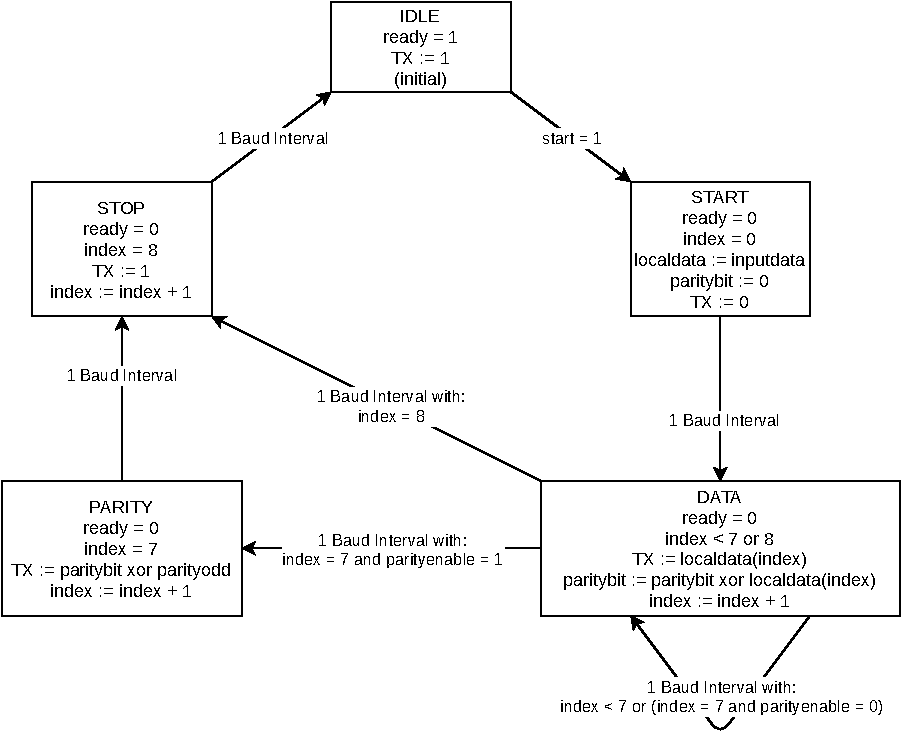
\includegraphics[width=\textwidth]{smtx}
	\caption{State machine of the TX block}
	\label{fig:smtx}
\end{figure}

\subsection{RX design}

The job of the RX block is to detect and receive a byte on the RX line, outputting the result to the controller logic. Its interface and internal registers are shown in figure \ref{fig:rx}.

When a low RX signal is detected in the idle state, the system goes into a pending state and waits for half a baud interval to sample the start bit and confirm this as an actual transmission. After that, the 8 data bits are sampled at the defined baud intervals. Finally the data is flushed to the controller and we return to the idle state. This state machine is represented in figure \ref{fig:smrx}.

\begin{figure}[h]
	\centering
	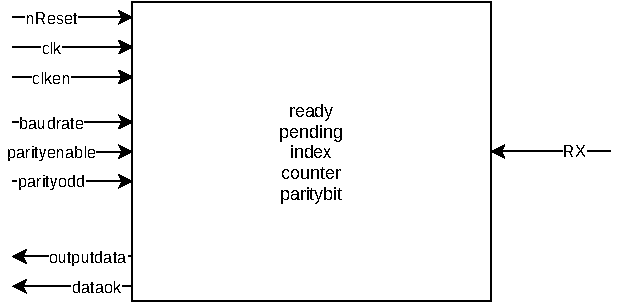
\includegraphics[width=.7\textwidth]{rx}
	\caption{Signals in the RX block}
	\label{fig:rx}
\end{figure}

\begin{figure}[h!]
	\centering
	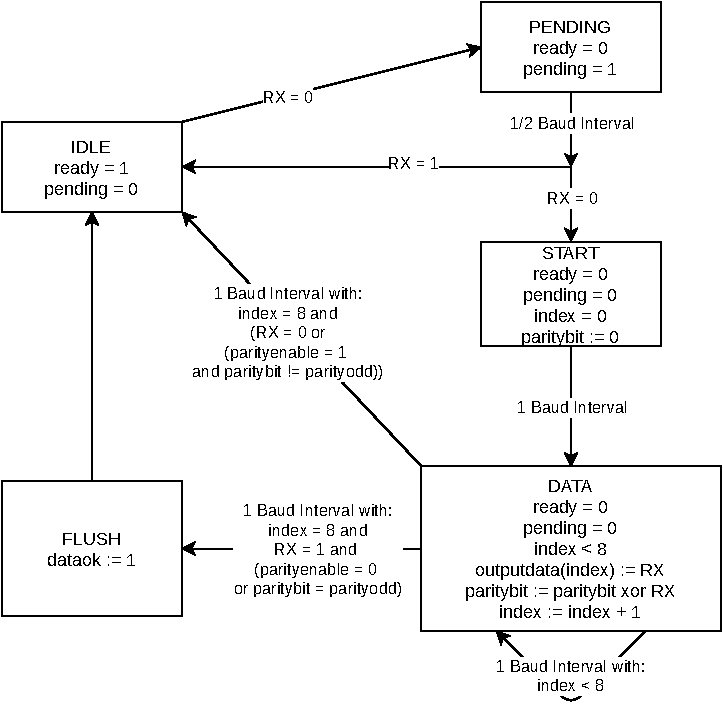
\includegraphics[width=.8\textwidth]{smrx}
	\caption{State machine of the RX block}
	\label{fig:smrx}
\end{figure}

\subsection{Timing of operations}

The following 3 figures show the rough timing of typical operations, with the most important interface and internal signal states. 

Figure \ref{fig:timerw} displays the timing of Avalon read and write operations. Reads are 1-wait, while writes are 0-wait.

Figure \ref{fig:timetx} shows the timing of a transmit operation, from the data write to the TXDATA register until the whole transmission has completed on the TX pin. The beginning of a second transmission is also shown.

Similarly, figure \ref{fig:timerx} shows the timing of a receive operation, and the data read of the received byte. The beginning of a second reception is also depicted.

\begin{figure}[h]
	\centering
	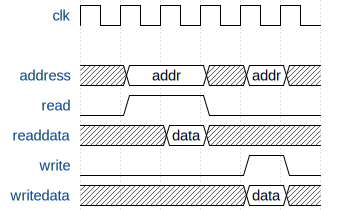
\includegraphics[width=.5\textwidth]{timings/read_write_ctrl}
	\caption{Timing of Avalon read \& write}
	\label{fig:timerw}
\end{figure}

\begin{figure}[h]
	\centering
	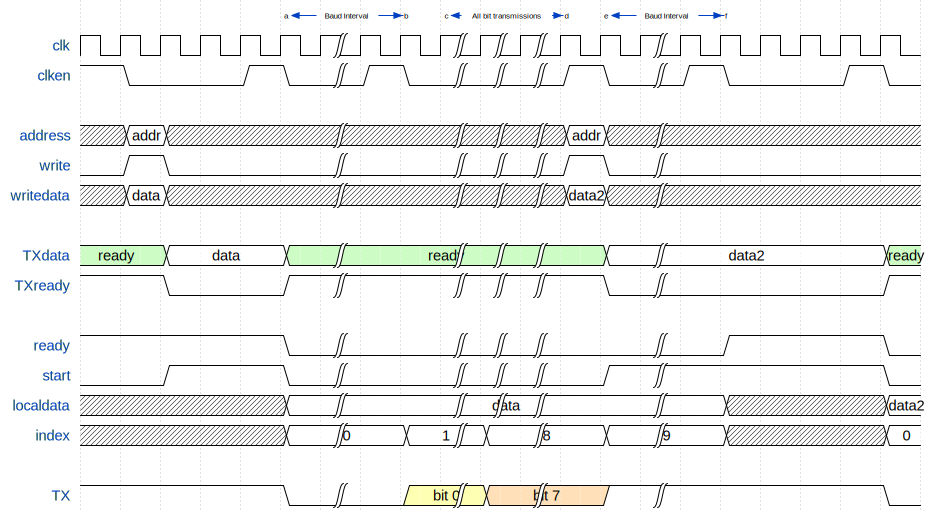
\includegraphics[width=\textwidth]{timings/TX}
	\caption{Timing of data transmission}
	\label{fig:timetx}
\end{figure}

\begin{figure}[p]
	\centering
	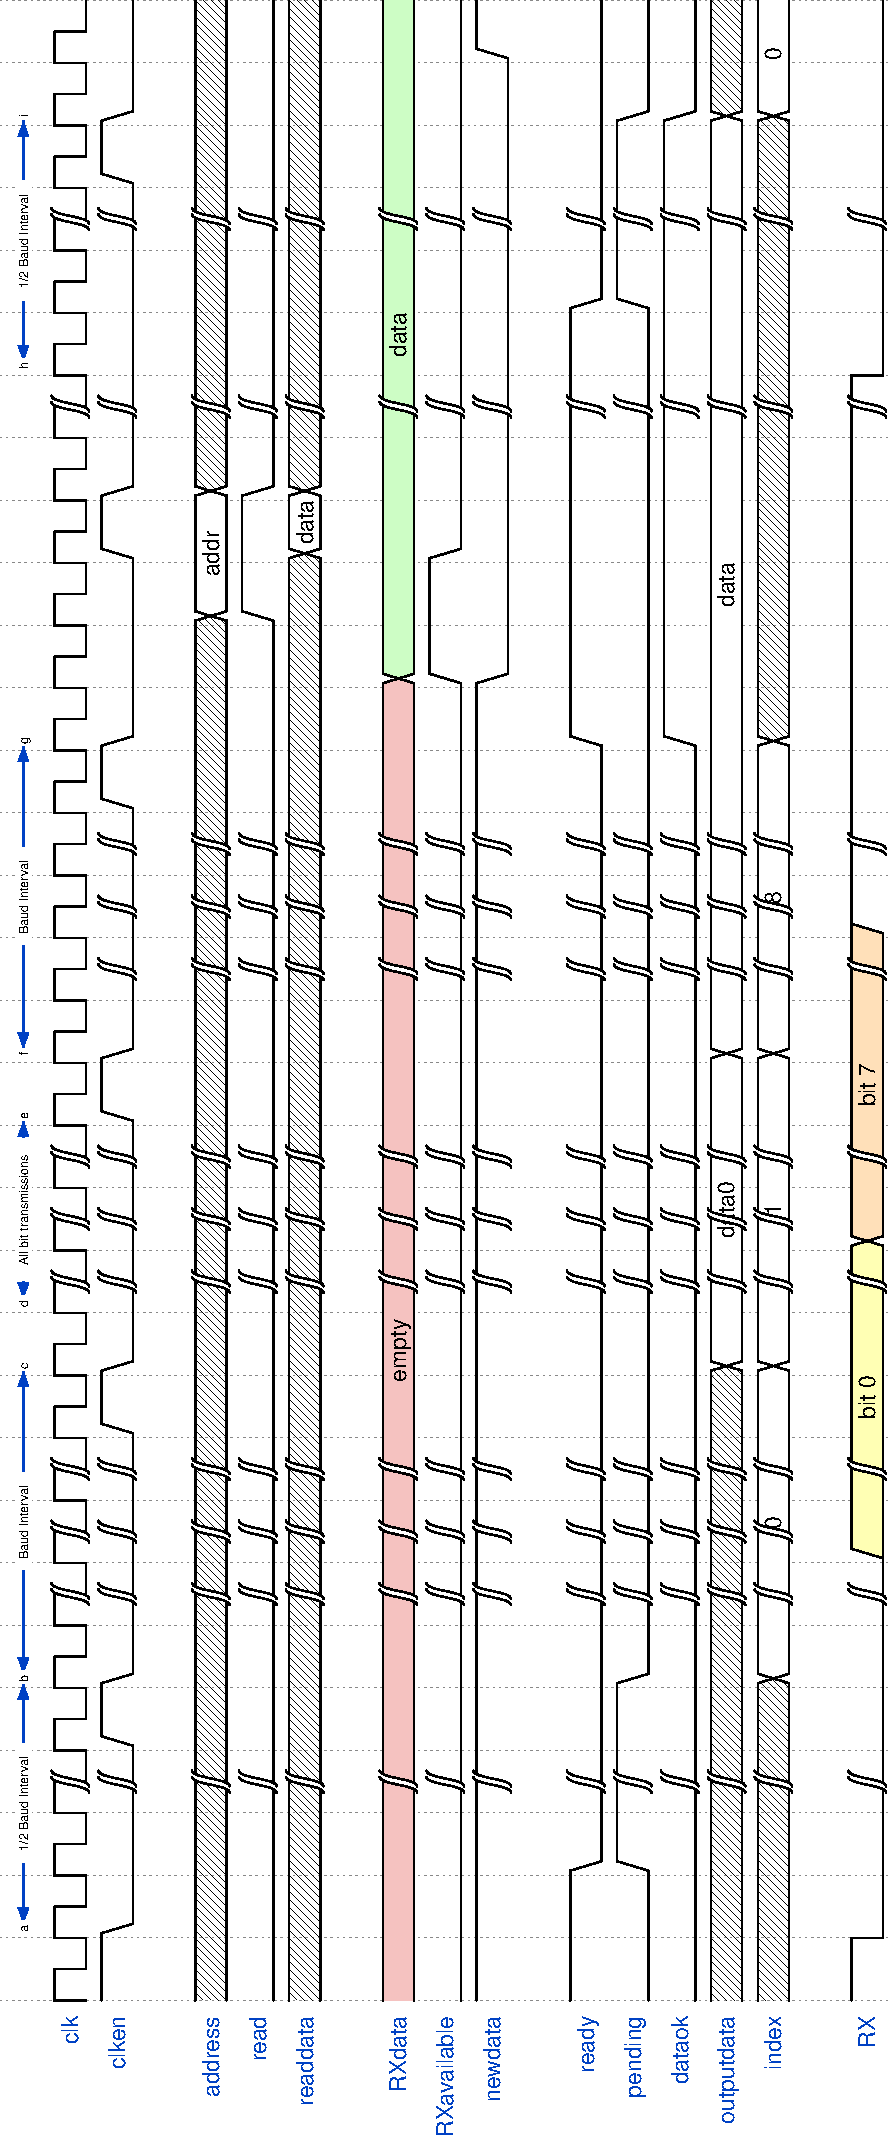
\includegraphics[width=.6\textwidth]{timings/RX_rot}
	\caption{Timing of data reception}
	\label{fig:timerx}
\end{figure}


\subsection{Implementation details}

All implementation files are found in the \texttt{hw/hdl/uart/comp} folder.

The TX and RX blocks are implemented respectively in the \texttt{uart\_tx.vhd} and \texttt{uart\_rx.vhd} files. All operations of the state machines (expect the detection of a reception start) are synchronous to the slow clock, and are implemented in a single process (with some helper procedures).

The clock divider is implemented in \texttt{clock\_divider.vhd}, and is a simple counter, regularly enabling the \texttt{clken} signal.

Finally the UART controller main logic is implemented in the \texttt{uart.vhd} file. It intantiates the 3 sub-entities, and defines two processes: one for Avalon slave writes and TX management, and the other for Avalon slave reads and RX management.

Testbenches can be found in the \texttt{hw/hdl/uart/testbench} folder. There is a testbench for each of these components.


\section{Calculator software}

In this section, we will describe the design and implementation of the ``calculator'' software. The goal is to create an application that can receive an arithmetic expression character-by-character, buffer it, parse it, evaluate it, and finally send back the result character-by-character. 

The code is separated into a UART driver managing the polling and buffers for the UART controller, and the main application logic implementing the calculator.

All the code can be found in the \texttt{sw/nios/application} folder.

\subsection{UART driver}

The UART driver has a large buffer for characters pending for transmission. It also stores a function pointer to a callback which is called for each received byte. The central function \texttt{run()} consists of an infinite loop, polling the UART controller's CTRLA register, and testing both the \texttt{RXavailable} and \texttt{TXready} flags.

If a some new received data is available, it is retrieved and the callback is called with this byte as argument. If the controller is ready for transmission, the next byte in the FIFO buffer is popped and sent to the controller.

The driver also supports managing the baud rate and parity settings.

\subsection{Main program}

The main program sets up the UART communication parameters, and registers a callback function for handling incoming characters. All characters except + and newline are buffered. When a + or newline arrives, the currently buffered character string is converted into a integer. Once we receive the newline, the result is calculated based on the 2 parsed integers, and a response string is formatted and buffered in the UART driver.


\section{Operation \& results}

For the operation, the controller and the minicom terminal were both set to a baud rate of 500kBaud, with a communication pattern of 7-bit data, even parity bit, and 1 stop bit (7E1).

The system works as expected. Expressions containing a single addition can be typed into the minicom terminal. These expressions are correctly sent over the UART pins to the FPGA. The connection is shown in figure \ref{fig:connection}. The calculator answers with a string which is correctly displayed on the host terminal. The obtained input/output is shown in figure \ref{fig:io}.

A demo video has also been submitted on Moodle, alongside this report and the source code.

\begin{figure}[h]
	\centering
	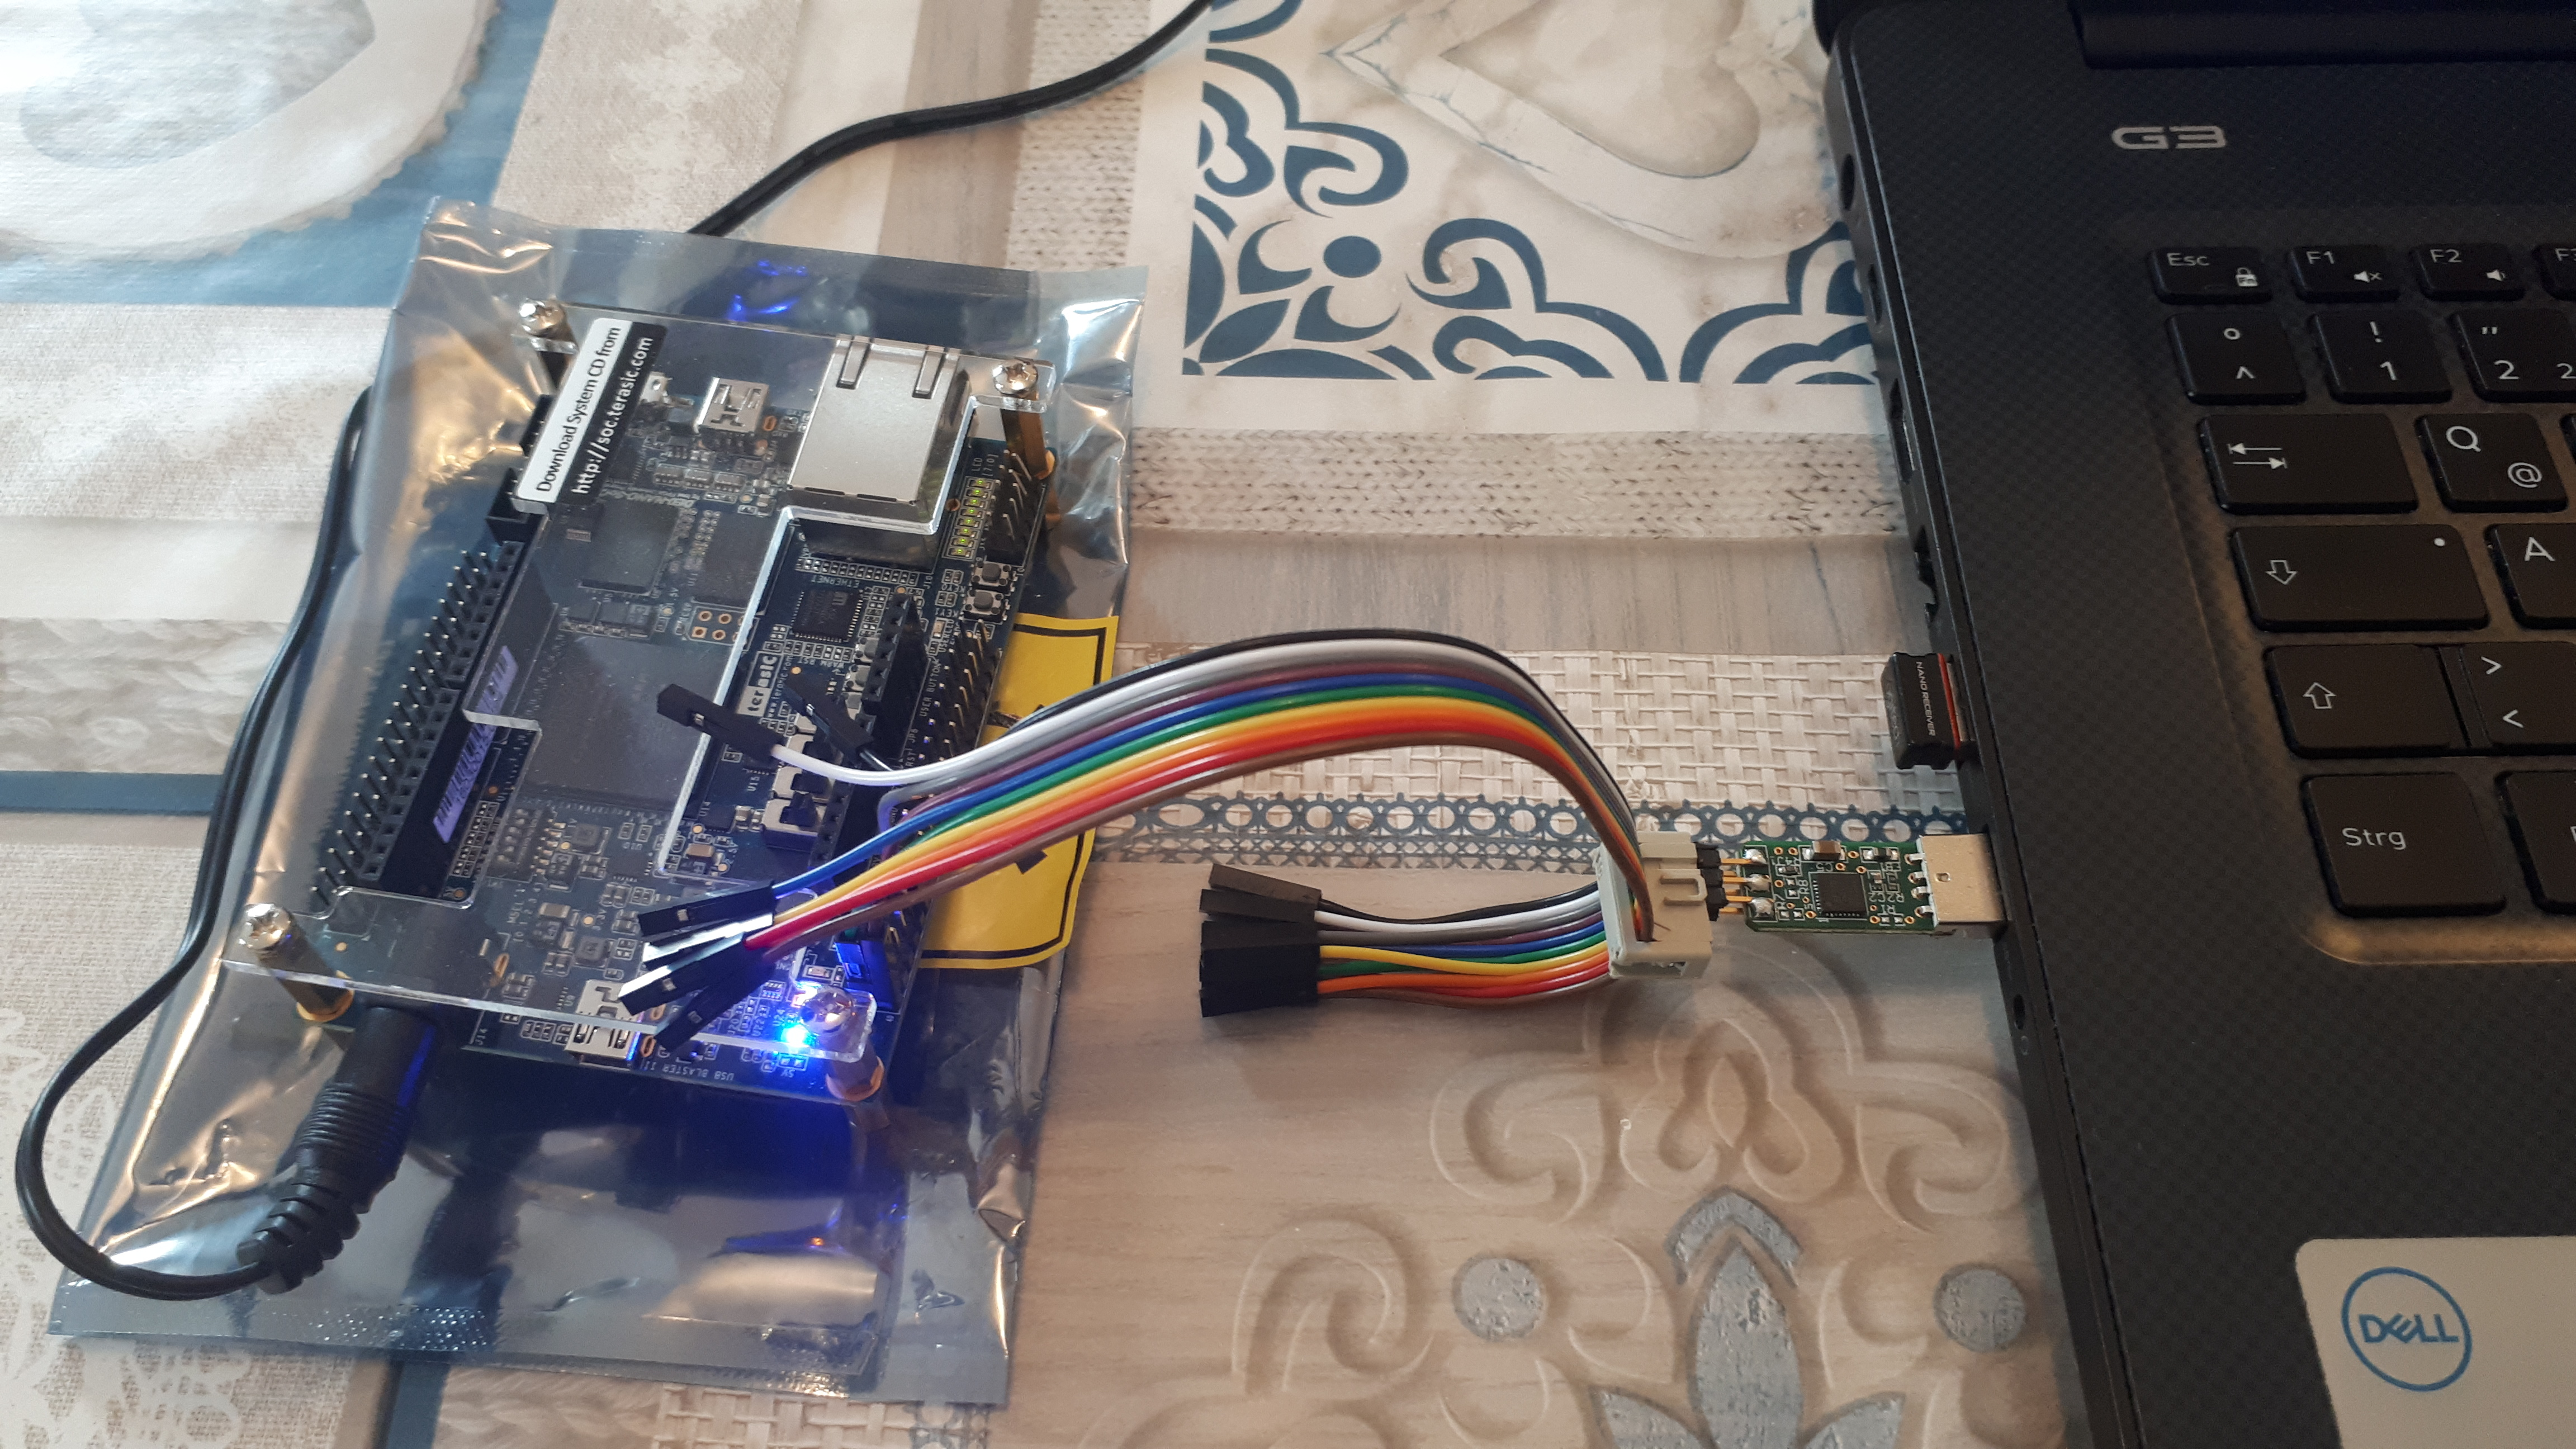
\includegraphics[width=\textwidth]{connections}
	\caption{Connections between the FPGA and the host computer}
	\label{fig:connection}
\end{figure}

\begin{figure}[h]
	\centering
	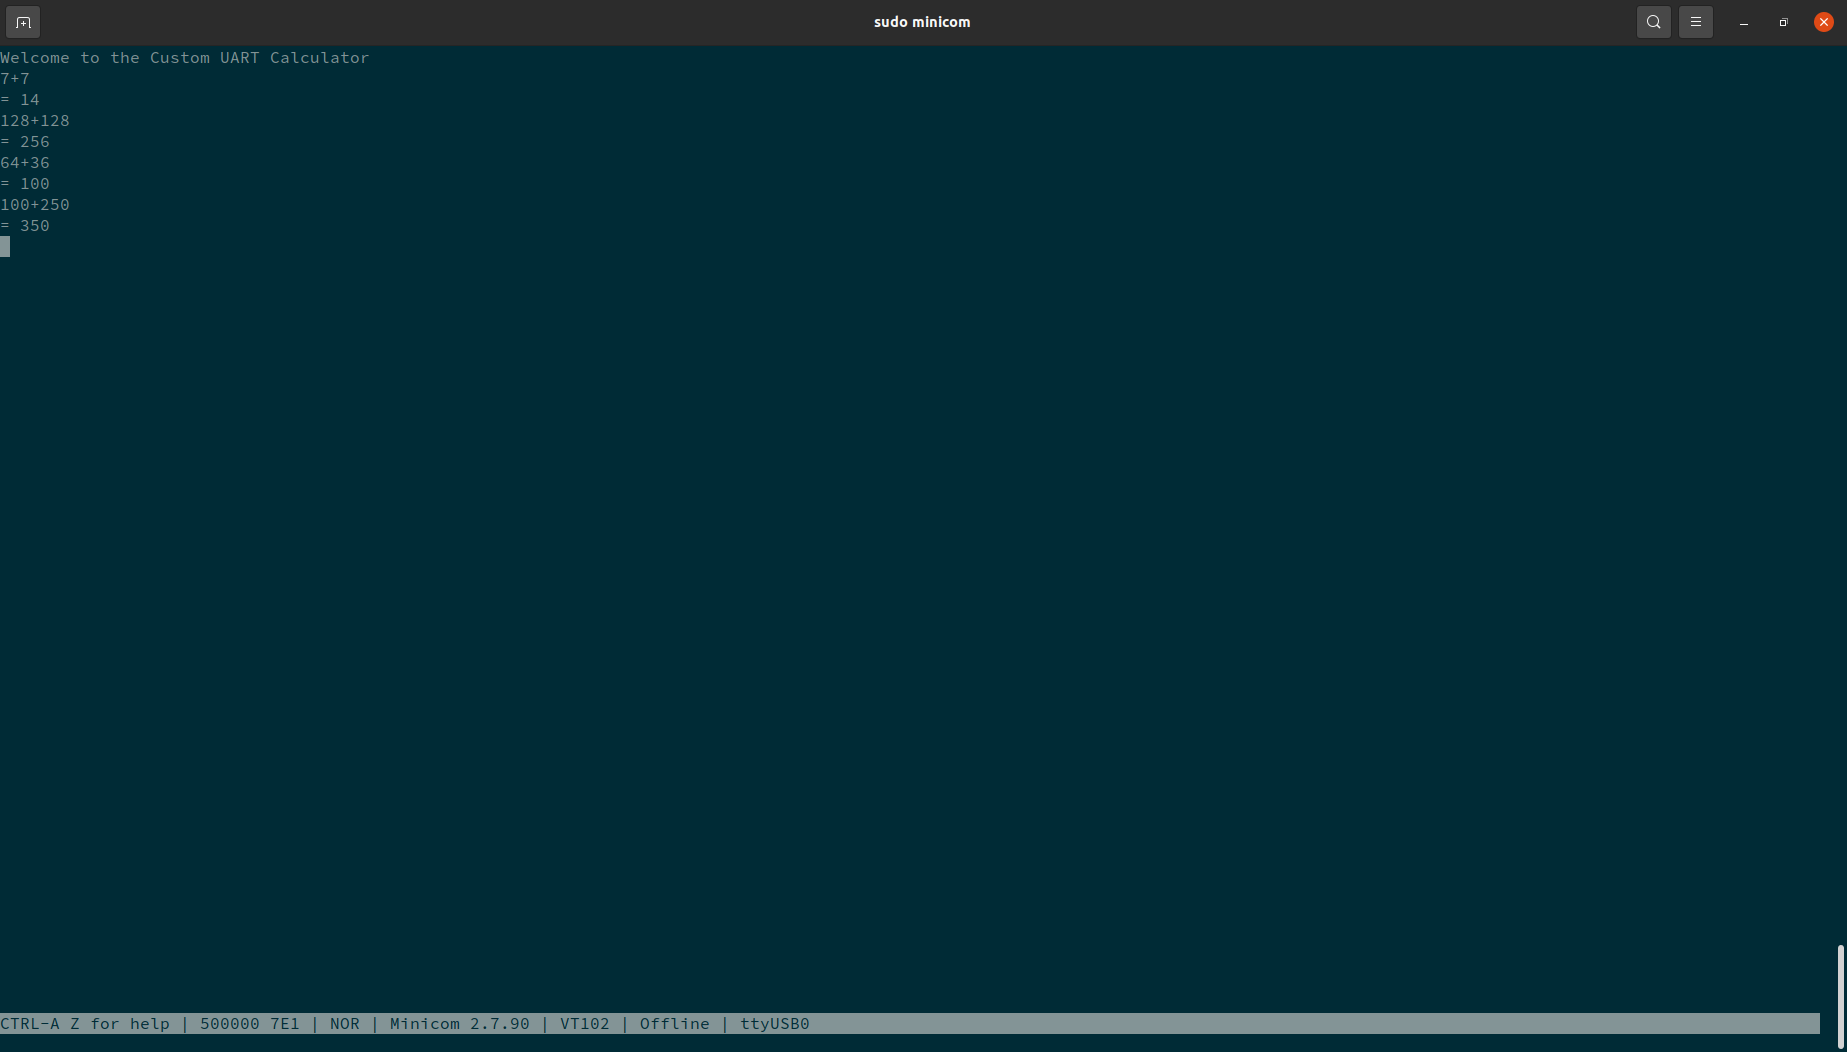
\includegraphics[width=\textwidth]{io}
	\caption{Input/output on the minicom terminal}
	\label{fig:io}
\end{figure}

\end{document}